%
% This is a borrowed LaTeX template file for lecture notes for CS267,
% Applications of Parallel Computing, UCBerkeley EECS Department.
% Now being used for CMU's 10725 Fall 2012 Optimization course
% taught by Geoff Gordon and Ryan Tibshirani.  When preparing
% LaTeX notes for this class, please use this template.
%
% To familiarize yourself with this template, the body contains
% some examples of its use.  Look them over.  Then you can
% run LaTeX on this file.  After you have LaTeXed this file then
% you can look over the result either by printing it out with
% dvips or using xdvi. "pdflatex template.tex" should also work.
%

\documentclass[UTF8,oneside]{article}

% \usepackage[UTF8,scheme=plain]{ctex}
\usepackage[AutoFakeBold,AutoFakeSlant,CJKecglue]{xeCJK}  % 载入 xeCJK以支持中文,支持伪粗体,伪斜体 , 去掉CJK 文字与西文字体间的空格
\usepackage[margin=1in]{geometry}
\usepackage{amsmath,amsthm,amssymb}
\usepackage{graphicx}
\usepackage{autobreak}
\usepackage{tikz}
\usepackage{array}
\usetikzlibrary{positioning} %为了实现相对位置的设定
\usepackage{xcolor} %为了实现不同的颜色
\setCJKmainfont{宋体}                                         % 设置中文中文字体
\setCJKmonofont{宋体}                                        % 设置中文等宽字体
% \setCJKsansfont{宋体}
% \setCJKmainfont{SimSun}[BoldFont=SimHei, ItalicFont=KaiTi]
\setlength{\oddsidemargin}{0.25 in}
\setlength{\evensidemargin}{-0.25 in}
\setlength{\topmargin}{-0.6 in}
\setlength{\textwidth}{6.5 in}
\setlength{\textheight}{8.5 in}
\setlength{\headsep}{0.75 in}
\setlength{\parindent}{0 in}
\setlength{\parskip}{0.1 in}

%
% ADD PACKAGES here:
%

\usepackage{amsmath,amsfonts,graphicx}

%
% The following commands set up the lecnum (lecture number)
% counter and make various numbering schemes work relative
% to the lecture number.
%
\newcounter{lecnum}
\renewcommand{\thepage}{\thelecnum-\arabic{page}}
\renewcommand{\thesection}{\thelecnum.\arabic{section}}
\renewcommand{\theequation}{\thelecnum.\arabic{equation}}
\renewcommand{\thefigure}{\thelecnum.\arabic{figure}}
\renewcommand{\thetable}{\thelecnum.\arabic{table}}

%
% The following macro is used to generate the header.
%
\newcommand{\lecture}[4]{
   \pagestyle{myheadings}
   \thispagestyle{plain}
   \newpage
   \setcounter{lecnum}{#1}
   \setcounter{page}{1}
   \noindent
   \begin{center}
   \framebox{
      \vbox{\vspace{2mm}
    \hbox to 6.28in { {\bf Fundamentals Of Information Science
	\hfill 2022 Spring} }
       \vspace{4mm}
       \hbox to 6.28in { {\Large \hfill   #2  \hfill} }
       \vspace{2mm}
       \hbox to 6.28in { {\it 学生: #3 \hfill 时间: #4} }
      \vspace{2mm}}
   }
   \end{center}
   \markboth{Lecture #1: #2}{Lecture #1: #2}

}
%
% Convention for citations is authors' initials followed by the year.
% For example, to cite a paper by Leighton and Maggs you would type
% \cite{LM89}, and to cite a paper by Strassen you would type \cite{S69}.
% (To avoid bibliography problems, for now we redefine the \cite command.)
% Also commands that create a suitable format for the reference list.
\renewcommand{\cite}[1]{[#1]}
\def\beginrefs{\begin{list}%
        {[\arabic{equation}]}{\usecounter{equation}
         \setlength{\leftmargin}{2.0truecm}\setlength{\labelsep}{0.4truecm}%
         \setlength{\labelwidth}{1.6truecm}}}
\def\endrefs{\end{list}}
\def\bibentry#1{\item[\hbox{[#1]}]}

%Use this command for a figure; it puts a figure in wherever you want it.
%usage: \fig{NUMBER}{SPACE-IN-INCHES}{CAPTION}
\newcommand{\fig}[3]{
			\vspace{#2}
			\begin{center}
			Figure \thelecnum.#1:~#3
			\end{center}
	}
% Use these for theorems, lemmas, proofs, etc.
\usepackage{amsthm}
\newtheorem*{Solution}{Solution}
\newtheorem{theorem}{Theorem}[lecnum]
\newtheorem{lemma}[theorem]{Lemma}

\newtheorem{proposition}[theorem]{Proposition}
\newtheorem{claim}[theorem]{Claim}
\newtheorem{corollary}[theorem]{Corollary}
\newtheorem{definition}[theorem]{Definition}
% \newenvironment{proof}{{\bf Proof:}}{\hfill\rule{2mm}{2mm}}

% **** IF YOU WANT TO DEFINE ADDITIONAL MACROS FOR YOURSELF, PUT THEM HERE:

\newcommand\E{\mathbb{E}}

\begin{document}
%FILL IN THE RIGHT INFO.
%\lecture{**LECTURE-NUMBER**}{**DATE**}{**LECTURER**}{**SCRIBE**}
\lecture{1}{Homework5}{华园(202000120027))}{2022.3.23}
%\footnotetext{These notes are partially based on those of Nigel Mansell.}

% **** YOUR NOTES GO HERE:

% Some general latex examples and examples making use of the
% macros follow.
%**** IN GENERAL, BE BRIEF. LONG SCRIBE NOTES, NO MATTER HOW WELL WRITTEN,
%**** ARE NEVER READ BY ANYBODY.

\section*{Problem 1.} % Don't be this informal in your notes!
Consider the discrete memoryless channel $Y_{i}=Z_{i} X_{i}$ with input alphabet $X_{i} \in\{-1,1\}$.\\
(a) What is the capacity of this channel when $\left\{Z_{i}\right\}$ is i.i.d. with
$$
Z_{i}=\left\{\begin{array}{cc}
1 & \mathrm{p}=0.5 \\
-1 & \mathrm{p}=0.5
\end{array}\right.
$$
(b) Now consider the channel with memory. Before transmission begins, $Z$ is randomly chosen and fixed for all time. Thus, $Y_{i}=Z X_{i}$.
What is the capacity if
$$
Z=\left\{\begin{array}{cc}
1 & \mathrm{p}=0.5 \\
-1 & \mathrm{p}=0.5
\end{array}\right.
$$
\begin{Solution}
\end{Solution}
(a)
\begin{center}
  \begin{tikzpicture}
\filldraw [black] (0,1.5) circle (0pt)--node[right=4pt,fill=white]{$-1$}(0,1.5);
\filldraw [black] (0,0) circle (0pt)--node[right=4pt,fill=white]{$1$}(0,0);

\filldraw [black] (-3,1.5) circle (0pt)--node[right=4pt,fill=white]{$-1$}(-3,1.5);
\filldraw [black] (-3,0) circle (0pt)--node[right=4pt,fill=white]{$1$}(-3,0);



\draw  [black,->](-2,1.5)--node[below=-5pt,fill=white]{$0.5$}(0,1.5);
\draw  [black,->](-2,1.5)--(0,0);
\draw  [black,->](-2,0)--node[below=-5pt,fill=white]{$0.5$}(0,0);
\draw  [black,->](-2,0)--node[below=-5pt,fill=white]{$0.5$}(0,1.5);
	\end{tikzpicture}\\
$$C=max(I(X;Y))=max[H(Y)-H(Y|X)]=1-1=0$$
\end{center}

(b)
\begin{center}
  \begin{tikzpicture}
\filldraw [black] (0,1.5) circle (0pt)--node[right=4pt,fill=white]{$-1$}(0,1.5);
\filldraw [black] (0,0) circle (0pt)--node[right=4pt,fill=white]{$1$}(0,0);
\filldraw [black] (-3,1.5) circle (0pt)--node[right=4pt,fill=white]{$-1$}(-3,1.5);
\filldraw [black] (-3,0) circle (0pt)--node[right=4pt,fill=white]{$1$}(-3,0);
\draw  [black,->](-2,1.5)--(0,1.5);
\draw  [black,->](-2,0)--(0,0);
\filldraw [black] (1,0.7) circle (0pt)--node[right=4pt,fill=white]{$or$}(1,0.7);
\filldraw [black] (5,1.5) circle (0pt)--node[right=4pt,fill=white]{$-1$}(5,1.5);
\filldraw [black] (5,0) circle (0pt)--node[right=4pt,fill=white]{$1$}(5,0);
\filldraw [black] (2,1.5) circle (0pt)--node[right=4pt,fill=white]{$-1$}(2,1.5);
\filldraw [black] (2,0) circle (0pt)--node[right=4pt,fill=white]{$1$}(2,0);
\draw  [black,->](3,1.5)--(5,0);
\draw  [black,->](3,0)--(5,1.5);
	\end{tikzpicture}\\
$$C=0.5max(I_1(X;Y))+0.5max(I_2(X;Y))=0.5+0.5=1$$
\end{center}


\section*{Problem 2.}
Neo receives a 7-bit string, $D_{1} D_{2} D_{3} D_{4} P_{1} P_{2} P_{3}$ from Morpheus, sent using a code, $\mathcal{C}$, with parity equations
$$
\begin{array}{l}
P_{1}=D_{1}+D_{2}+D_{3} \\
P_{2}=D_{1}+D_{2}+D_{4} \\
P_{3}=D_{1}+D_{3}+D_{4}
\end{array}
$$
(a)Write down the generator matrix, $G$, for $\mathcal{C}$.
(b)Write down the parity check matrix, $H$, for $\mathcal{C}$.
(c)If Neo receives 1000010 and does maximum-likelihood decoding on it, what would his estimate of the data transmission $D_{1} D_{2} D_{3} D_{4}$ from Morpheus be? For your convenience, the syndrome $s_{i}$ corresponding to data bit $D_{i}$ being wrong are given below, for $i=1,2,3,4$ :
$$
s_{1}=(111)^{T}, s_{2}=(110)^{T}, s_{3}=(101)^{T}, s_{4}=(011)^{T} .
$$
(d)If Neo uses syndrome decoding for error correction, how many syndromes does he need to compute and store for this code, including the syndrome with no errors?
\begin{Solution}
\end{Solution}
(a)because $P_{1}=D_{1}+D_{2}+D_{3},P_{2}=D_{1}+D_{2}+D_{4},P_{3}=D_{1}+D_{3}+D_{4}$,we can get:\\
\begin{center}
$[D_1,D_2,D_3,D_4]·G=[D_{1}, D_{2}, D_{3}, D_{4}, P_{1}, P_{2}, P_{3}]$\\
$$G=\left[\begin{array}{lllllll}
1 & 0 & 0 & 0 & 1 & 1 & 1 \\
0 & 1 & 0 & 0 & 1 & 1 & 0 \\
0 & 0 & 1 & 0 & 1 & 0 & 1 \\
0 & 0 & 0 & 1 & 0 & 1 & 1
\end{array}\right]
$$
\end{center}

(b)According to G,we can also get:
\begin{center}
$H=\left[\begin{array}{lllllll}
1 & 1 & 1 & 0 & 1 & 0 & 0 \\
1 & 1 & 0 & 1 & 0 & 1 & 0 \\
1 & 0 & 1 & 1 & 0 & 0 & 1
\end{array}\right]
$
\end{center}
(c)
\begin{center}
$$
S=H \cdot r^{T}=\left[\begin{array}{lllllll}
1 & 1 & 1 & 0 & 1 & 0 & 0 \\
1 & 1 & 0 & 1 & 0 & 1 & 0 \\
1 & 0 & 1 & 1 & 0 & 0 & 1
\end{array}\right] \cdot\left[\begin{array}{l}
1 \\
0 \\
0 \\
0 \\
0 \\
1 \\
0
\end{array}\right]=\left(\begin{array}{lll}
1 & 0 & 1
\end{array}\right)^{T}
$$\\
Therefore, we believe that $D_{3}$ occurred an error in the transmission process\\
$$D_1D_2D_3D_4=1010$$
\end{center}
(d)
If there is only one error in 7-bit coding, there are 7 cases in total. Plus the case that there is no error, a total of 8 syndromes are required
\section*{Problem 3.}
For any linear block code over $\mathbb{F}_{2}$ with minimum Hamming distance at least $2 \mathrm{t}+1$ between codewords, show that:
$$
2^{n-k} \geq 1+\left(\begin{array}{l}
n \\
1
\end{array}\right)+\left(\begin{array}{l}
n \\
2
\end{array}\right)+\ldots+\left(\begin{array}{l}
n \\
t
\end{array}\right) .
$$
Hint: How many errors can such a code always correct?\\
For each $(n, k, d)$ combination below, state whether a linear block code with those parameters exists or not. Please provide a brief explanation for each case: if such a code exists, give an example; if not, you may rely on a suitable necessary condition.\\
(a) $(31,26,3):$ Yes / No\\
(b) $(32,27,3)$ : Yes / No\\
(c) $(43,42,2)$ : Yes / No\\
(d) $(27,18,3)$ : Yes / No\\
(e) $(11,5,5)$ : Yes / No\\
\begin{Solution}
\end{Solution}
最小汉明顿距离为2t+1的线性分组码可以纠正至多t个错误,码字长度为n,当发生a个错误时,有$C_{n}^{a}$种情况,所以全部可纠正错误的个数为: 
$$\left(\begin{array}{l}
n \\
1
\end{array}\right)+\left(\begin{array}{l}
n \\
2
\end{array}\right)+\ldots+\left(\begin{array}{l}
n \\
t
\end{array}\right) .$$
sysndromes 可以代表的错误个数为:
$$2^{n-k}-1$$
减一代表减去全部传输正确的情况,即S=0的情况。\\
为了在解码过程中能够根据sysndromes纠正错误,所以sysndromes所能代表的错误个数必须要大于或者等于可以纠正的错误的个数,因此满足以下不等式:
$$
2^{n-k}-1 \geq \left(\begin{array}{l}
n \\
1
\end{array}\right)+\left(\begin{array}{l}
n \\
2
\end{array}\right)+\ldots+\left(\begin{array}{l}
n \\
th
\end{array}\right) .
$$
从而可以获得:
$$
2^{n-k} \geq 1+\left(\begin{array}{l}
n \\
1
\end{array}\right)+\left(\begin{array}{l}
n \\
2
\end{array}\right)+\ldots+\left(\begin{array}{l}
n \\
t
\end{array}\right) .
$$\\
(a)YES,\quad$\frac{d-1}{2}=1$\;and\;$2^{n-k}-1=31=n$,this code exists and the example is Hamming code.\\
(b)NO,\quad$\frac{d-1}{2}=1$\;and\;$2^{n-k}-1=31<n$,this code  doesn't exist. \\
(c)NO,\quad$\frac{d-1}{2}=0.5$,thus this code can not correct the error,this code doesn't exist\\
(d)YES,\quad$\frac{d-1}{2}=1$\;and\;$2^{n-k}-1=511>n$,this code exists\\
(e))NO,\quad$\frac{d-1}{2}=2$\;and\;$2^{n-k}-1=63<n+n(n-1)/2=66$,this code  doesn't exist. \\
\section*{Problem 4.}
(a) List the elements in Galois field $G F\left(2^{3}\right)$ of primitive $x^{3}+x+1$ as successive powers of the primitive element $x$.\\
(b) Construct a Reed-Solomon Code with $n=5$ and $k=3$, and use this code to encode a sequence 001010011 (first converting 001,010,011 to elements in $\left.G F\left(2^{3}\right)\right)$. Please show how the codeword is generated.
\begin{Solution}
\end{Solution}
(a)
\begin{align*}
\alpha^0&=\quad\quad\quad\quad1\\
\alpha^1&=\quad\quad\, x\\
\alpha^2&=x^2\\
\alpha^3&=\quad\quad \,x +\, 1\\
\alpha^4&=x^2+x\\
\alpha^5&=x^2+x+1\\
\alpha^6&=x^2\quad+\;\;\;1\\
\alpha^7&=\quad\quad\quad\quad1\\

\end{align*}
(b)
\begin{center}
$\beta_1=0\qquad \beta_2=1\qquad\beta_3=x\qquad\beta_4=x^2$\\
$\beta_5=x+1\qquad \beta_6=x^2+x\qquad\beta_7=x^2+x+1\qquad\beta_8=x^2+1$\\
\end{center}
$$A=\left[\begin{array}{ccccc}1 & 1 & 1 & 1 & 1 \\ \beta_{1} & \beta_{2} & \beta_{3} & \beta_{4} & \beta_{5} \\ \beta_{1}^{2} & \beta_{2}^{2} & \beta_{3}^{2} & \beta_{4}^{2} & \beta_{5}^{2}\end{array}\right]$$
\begin{center}
$(001,010,011)\rightarrow(1,x,x+1)$
\end{center}
$$M=\left[\begin{array}{lll}1 & \mathrm{x} & x+1\end{array}\right]$$
Accoring to C=M·A,  we can get:
\begin{align*}
C_1&=m_0+m_1\beta_1+m_2\beta_1^2=1\\
C_2&=m_0+m_1\beta_2+m_2\beta_2^2=0\\
C_3&=m_0+m_1\beta_3+m_2\beta_3^2=x\\
C_4&=m_0+m_1\beta_4+m_2\beta_4^2=x+1\\
C_5&=m_0+m_1\beta_5+m_2\beta_5^2=x+1\\
\end{align*}
% **** THIS ENDS THE EXAMPLES. DON'T DELETE THE FOLLOWING LINE:
\begin{center}
so the code is (1,0,x,x+1,x+1)
\end{center}
\end{document}





h'j'h